\section{Exercise 2: Lanczos algorithm}
The Hamiltonian of the fermionic chain is given by
\begin{align}
    \mathcal{H} = - t \sum^N_{i=1} \left( | i \rangle \langle i+1| + | i+ 1\rangle \langle i |  \right) +  \epsilon | N/2 \rangle \langle N/2|
\end{align}

\subsection{Implementation of the Lanczos algorithm}
The algorithm is implemented according to the lecture (script beckmann p.30).

\subsection{Ground state and ground energy}
For a chain of $N=6$ lattice sites the Hamiltonian is given by
\begin{align}
    \mathcal{H} = 
    \begin{pmatrix}
        0&-t&0&0&0& \fcolorbox{red}{white}{-t} \\
        -t&0&-t&0&0&0 \\
        0&-t&\epsilon&-t&0&0 \\
        0&0&-t&0&-t&0 \\
        0&0&0&-t&0&-t \\
        \fcolorbox{red}{white}{-t}&0&0&0&-t&0 
    \end{pmatrix}
\end{align}
The entries marked in red represent the periodic boundary condition $| N+1 \rangle = | N\rangle$. The ground state energy $E_0$ in dependence of the energy $\epsilon$ of the impurity is shown in Fig.\ref{fig:ex01_1}. For $\epsilon < 0$ the ground state energy tends towards $\epsilon$, for $\epsilon > 0$ the impurity has no impact on the ground state energy.\\
The particle density for $\epsilon = -20,2,20$ is shown in Fig.\ref{fig:ex01_2}. For very small values the particles are located at the impurity, for large values the impurity has a repulsive character, so no particles are located there. For $\epsilon = 0$ the particles are uniformly distributed.

\begin{figure}[h]
    \centering
    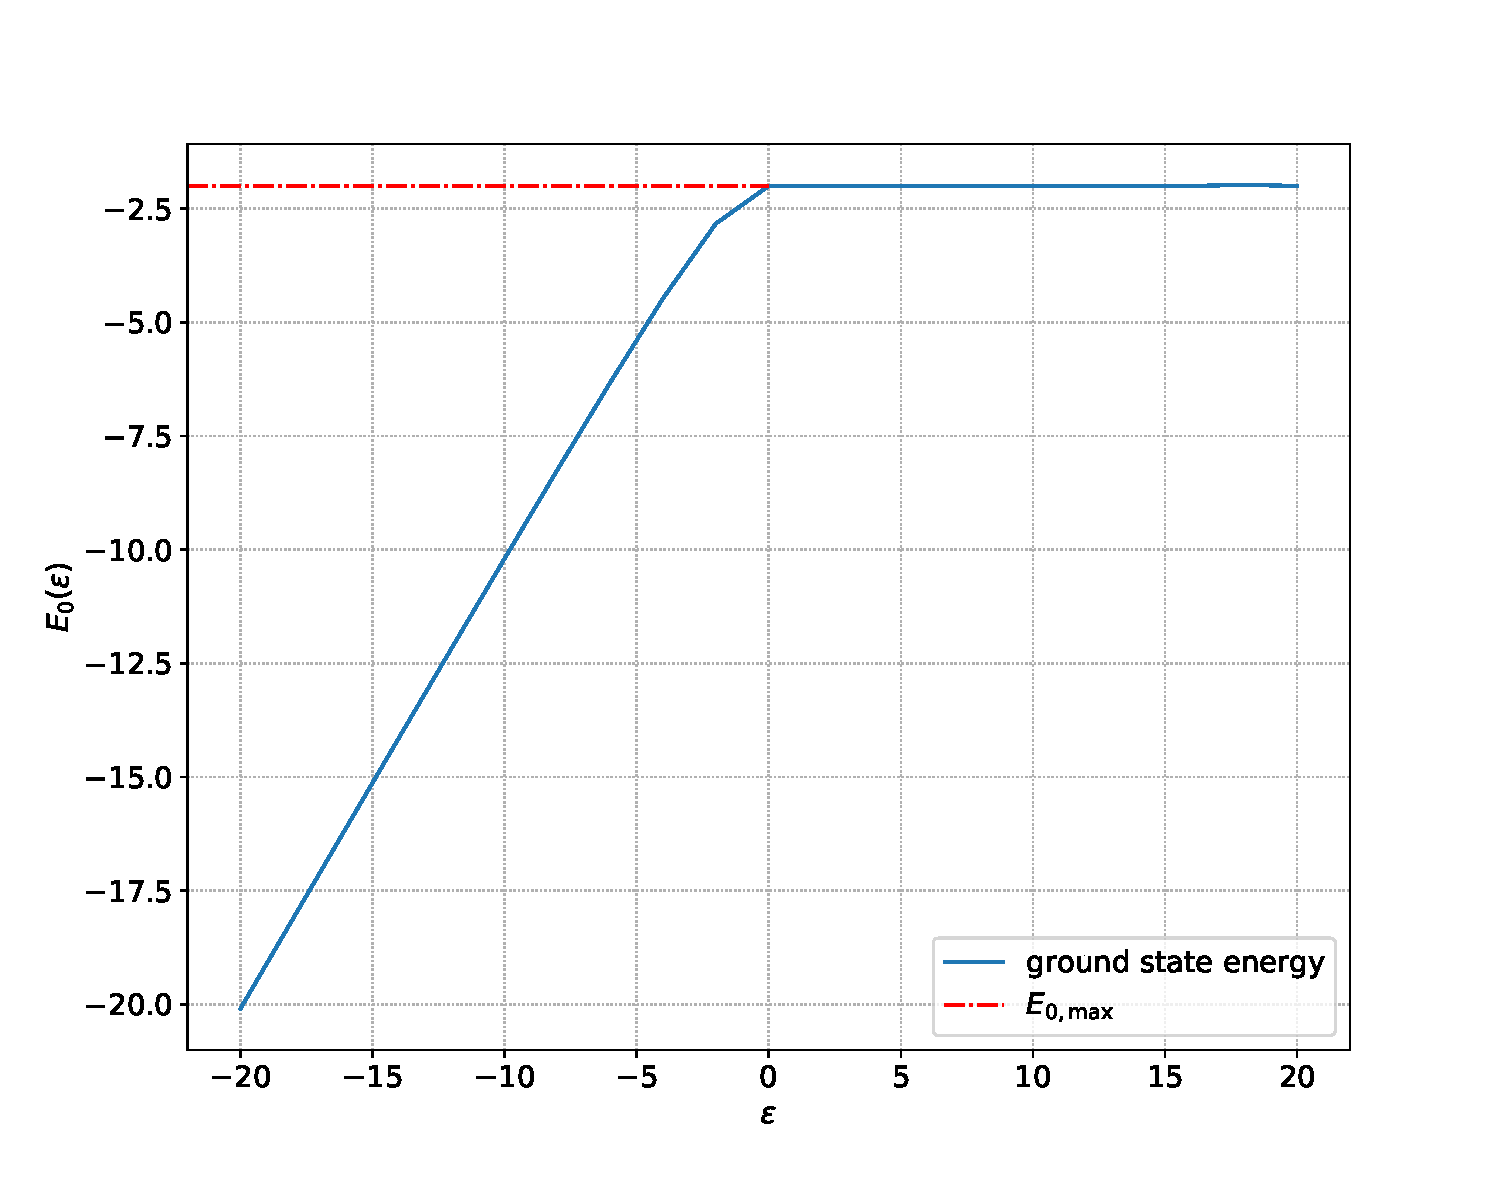
\includegraphics[width=\textwidth]{../code/build/ex01_gse.pdf}
    \caption{Ground state energy for different $\epsilon$'s. }
    \label{fig:ex01_1}
\end{figure}

\begin{figure}[h]
    \centering
    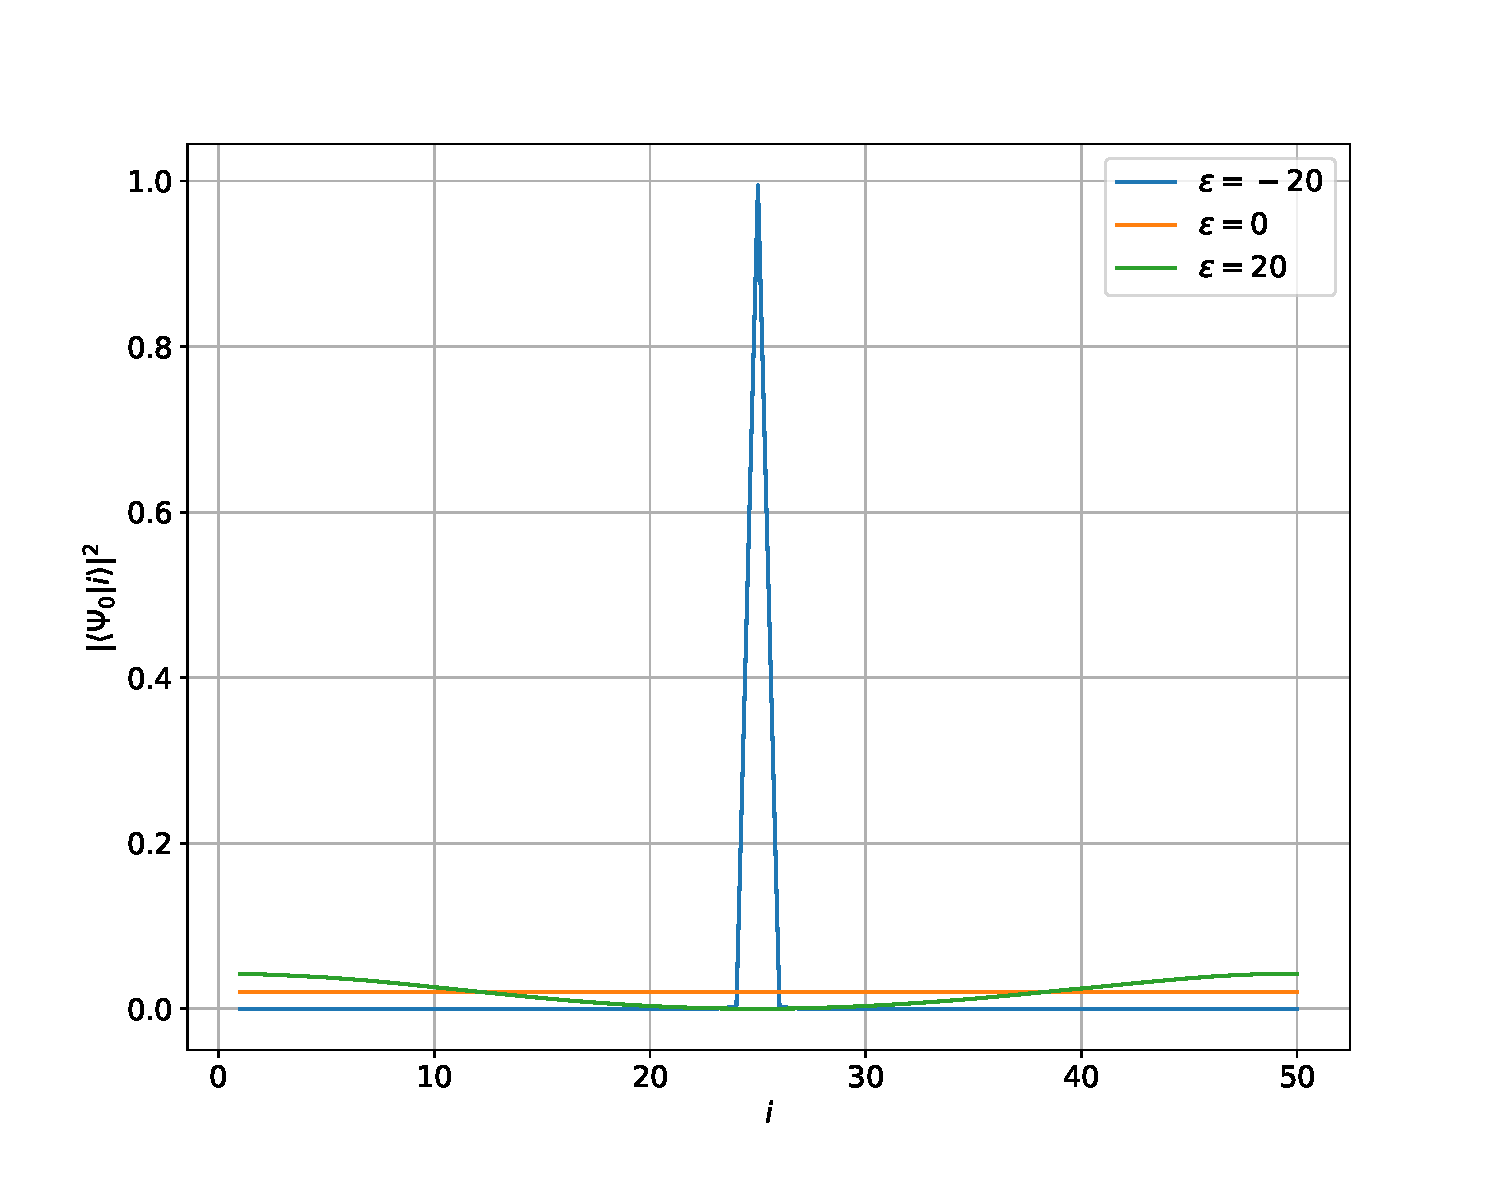
\includegraphics[width=\textwidth]{../code/build/ex01_pd.pdf}
    \caption{Particle density for $\epsilon = -20, 0, 20$.}
    \label{fig:ex01_2}
\end{figure}

\subsection{ Organization of storage }
Since $\mathcal{H}$ only contains a small number of non-zero elements, a sparse-matrix could be used.